\documentclass{standalone}
\usepackage{tikz}
\usepackage{pgfplots}
\usepackage{mathtools}

\pgfplotsset{compat = newest}
\usetikzlibrary{decorations.markings,arrows.meta}
\usepgfplotslibrary{fillbetween}

\begin{document}
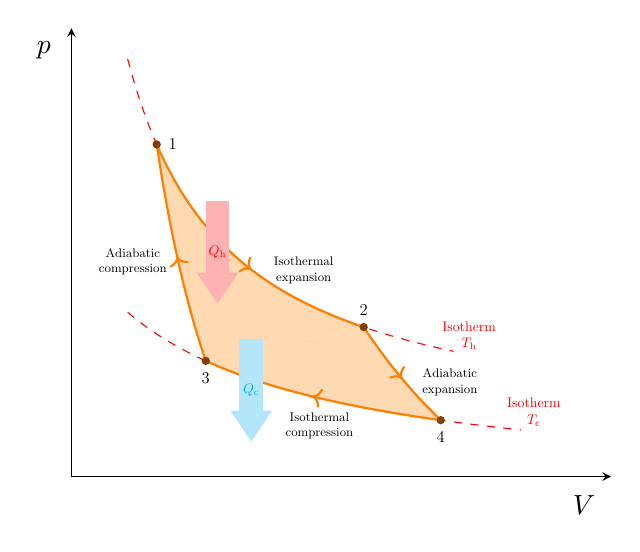
\begin{tikzpicture}[scale=1, every node/.style={scale=0.5}]
  \begin{axis}[
      axis lines=left,
      xmin=0.2,xmax=2.6,
      ymin=-0.2,ymax=2.4,
      xtick=\empty, ytick=\empty,
      y label style={scale=2,at={(axis description cs:-0.02,0.95)},rotate=270},
      x label style={scale=2,at={(axis description cs:0.95,-0.02)}},
      ylabel={$p$},
      xlabel={$V$},
    ]
    % \node [below left] at (axis cs:0,-1) {$-1$};
    % \node [above left] at (axis cs:0,1) {$1$};
    % \addplot[thick,orange,samples=100,smooth,domain=1.25:2*pi-2,
    %   postaction={decorate},
    %   decoration={markings,
    %       mark=at position 0.25 with {\arrow{stealth}}}] {1/x};

    \addplot [thin,samples=100,smooth,red,dashed,domain=0.45:1.9] {1/x} node[pos=1.03,above,text width=1.75cm,align=center]{Isotherm $T_\text{h}$};
    \addplot [thin,samples=200,smooth,red,dashed,domain=0.45:2.2]{1/(x+0.5)-0.3} node[pos=1.03,above,text width=1.75cm,align=center]{Isotherm $T_\text{c}$};

    \addplot [thick,samples=100,smooth,orange,domain=0.5794:1.5,name path=A] {1/x}; % isothermal expansion
    \addplot [thick,samples=200,smooth,orange,domain=1.5:1.8426,name path=B] {3.6/(x-0.15)-2}; % adiabatic expansion
    \addplot [thick,samples=200,smooth,orange,domain=0.7976:1.8426,name path=C] {1/(x+0.5)-0.3}; % isothermal compression
    \addplot [thick,samples=200,smooth,orange,domain=0.5794:0.7976,name path=D] {1.6/(x-0.15)-2}; % adiabatic compression

    \addplot[orange!30] fill between[of = A and D];
    \addplot[orange!30] fill between[of = C and B];

    % Points
    \fill[orange!50!black] (0.5794,1/0.5794)  circle[radius=1.5pt] node[black,font=\large] at (axis cs:0.65,1/0.5794) {1};
    \fill[orange!50!black] (1.5,1/1.5)  circle[radius=1.5pt] node[black,font=\large] at (axis cs:1.5,1/1.5+0.1)  {2};
    \fill[orange!50!black] (0.7976,1/1.2976-0.3)  circle[radius=1.5pt] node[black,font=\large] at (axis cs:0.7976,1/1.2976-0.4)  {3};
    \fill[orange!50!black] (1.8426,1/2.3426-0.3)  circle[radius=1.5pt] node[black,font=\large] at (axis cs:1.8426,1/2.3426-0.4)  {4};

    % Labels
    \node [below left,text width=2cm,align=center,font=\small] at (axis cs:1.43,1.1) {Isothermal expansion};
    \node [below left,text width=2cm,align=center,font=\small] at (axis cs:2.08,0.45) {Adiabatic expansion};
    \node [below left,text width=2cm,align=center,font=\small] at (axis cs:1.5,0.2) {Isothermal compression};
    \node [below left,text width=2cm,align=center,font=\small] at (axis cs:0.67,1.15) {Adiabatic compression};

    % Arrows diagram
    \draw[->,orange,thick] (1.0,1/1.0)--(1.0001,1/1.0001);
    \draw[->,orange,thick] (1.671,3.6/1.521-2)--(1.6711,3.6/1.5211-2);
    \draw[->,orange,thick] (1.2702,1/1.7702-0.3)--(1.2701,1/1.7701-0.3);
    \draw[->,orange,thick] (0.6701,1.6/0.5201-2)--(0.67,1.6/0.52-2);

    % Arrows - heat
    \draw[red!30, arrows={-Triangle[length=4mm,width=5mm]},line width=3mm]  (0.85,1.4) --node[red]{$Q_\text{h}$} (0.85,0.8);
    \draw[cyan!30, arrows={-Triangle[length=4mm,width=5mm]},line width=3mm]  (1,0.6) --node[cyan]{$Q_\text{c}$} (1,0);
  \end{axis}
  % [
  %   % Corner style
  %   corner/.style={
  %       circle,
  %       fill,
  %       inner sep=1pt},
  %   % Line with Arrow style
  %   arrowline/.style={
  %       thick,
  %       postaction = decorate,
  %       decoration = {markings,
  %           mark = at position .6 with \arrow{latex}
  %         }
  %     },
  %   % Pin style
  %   every pin/.style = {
  %       black!80,
  %       inner sep = 1mm,
  %       align = center,
  %       font = \footnotesize,
  %       pin edge = {-latex, thin, line to}},
  % ]

  % % Draw axis with labels
  % \draw [latex-latex] (0,6)  |- (8,0)
  % node [pos=.95,below] {Volume}
  % node [pos=0.07,above,rotate=90] {Pressure};

  % % Cycle corners
  % \node[corner,
  %   label = {left:$1$}] (1) at (2,5){} ;

  % \node[corner,
  %   label = {right:$2$}] (2) at (4.5,4){} ;

  % \node[corner,
  %   label = {right:$3$}] (3) at (5.5,1.5){} ;

  % \node[corner,
  %   label = {below left:$4$}] (4) at (2.5,2.5){} ;

  % % Curved lines
  % \draw [arrowline,blue!70] (1) to [bend right = 15]
  % node [pos = .4, pin = {45:Isothermal\\Expansion}] {} (2);

  % \draw [arrowline,red!70 ] (2) to [bend right = 15]
  % node [pos = .4, pin = {right:Adiabatic\\Expansion}] {}(3);

  % \draw [arrowline,blue!70] (3) to [bend left  = 15]
  % node [pos = .4, pin = {below:Isothermal\\Compression}] {} (4);

  % \draw [arrowline,red!70 ] (4) to [bend left  = 15]
  % node [pos = .4, pin = {260:Adiabatic\\Compression}] {} (1);

\end{tikzpicture}

\end{document}